\documentclass{article}
\usepackage{graphics}
\usepackage{epsfig}
\usepackage{natbib}
\usepackage{amsmath} %package for maths

%%%%%%%%%%%%%%%%%%%%%%%%%%%%%%
\begin{document}

    \title{Un documento sin ortografia}
    \author{Unautor sinortografia \and Uncoautor sincerebro}
    \date{Primera version Agosto 26. Ultima version \today}
    \maketitle

    %%%%%%%%%%%%%%%%%%%%%%%%%%%%%%
    \begin{abstract}
        Nunca aprendi ortografia.
    \end{abstract}

\newpage
\tableofcontents
\listoftables
\listoffigures

\newpage
%%%%%%%%%%%%%%%%%%%%%%%%%%%%%%
\section{Introduccion}\label{sec.intro}
    Siempre quise aprender a escribir.

    \begin{table}[h]
        \centering
        \caption[Nr of news by section and authored]{Nr of news by section and authored}
        \begin{tabular}{lrr}
        \hline
        Newspaper section & No. of news & Nr. of authored news \\
        Economy & 1,015 & 243 \\
        Editorial - Opinion & 439 & 288 \\
        \hline
        \multicolumn{3}{p{0.70\textwidth}}{\footnotesize{\emph{Note}: Authored news correspond to those where the name of author is published. News without author are assumed to be authored by newspaper staff. Editorial - opinion section include editorials and op-eds, op-eds are those which include the name of the author.}}\\
        \end{tabular}
        \label{tab:news.description}
    \end{table}

%%%%%%%%%%%%%%%%%%%%%%%%%%%%%%
\section{Explicacion de la introduccion}\label{sec.intro.explicacion}
    Nunca aprendi ortografia.

    \begin{figure}[h]
    \centering
    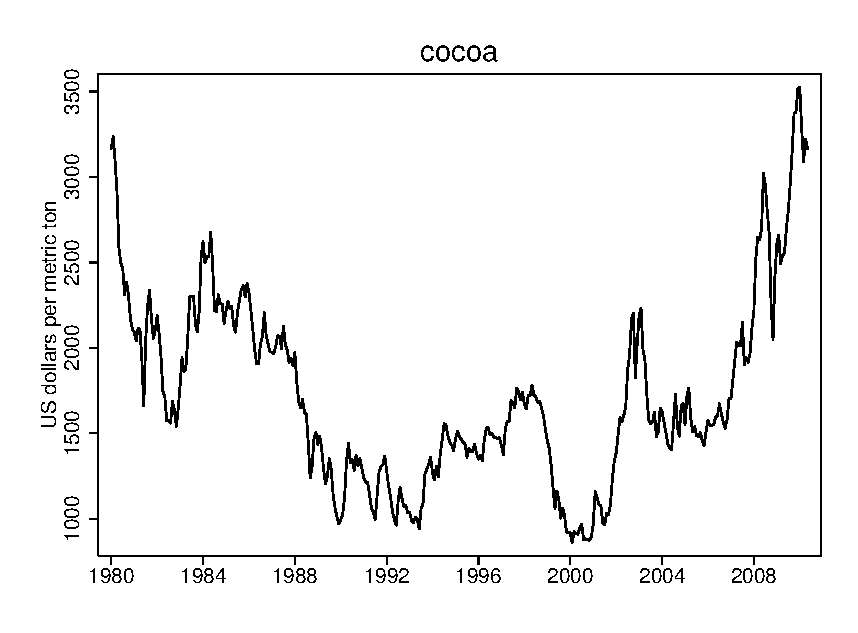
\includegraphics[width=0.8\textwidth, angle=0]{acocoa.eps}
    \caption{Cacao}
    \label{cacao}
    \end{figure}

%%%%%%%%%%%%%%%%%%%%%%%%%%%%%%
\section{Algunas f\'ormulas}\label{sec.intro.explicacion}

    $\sum_{i_1}^{100} a_i$
    
    \begin{align}
      a &= b \\
      aaa &= bbb
    \end{align}
    
    $$
    \begin{matrix}
    a & b \\
    c & d \\
    \end{matrix}
    $$

\section{Conclusion}\label{sec.conclusion}
    Mejor no escribo mas como en seccion \ref{sec.intro} y subseccion \ref{sec.intro.explicacion}. Por favor no olvidar \cite{ben1994inventory}

\newpage
    \bibliographystyle{chicago}
    \bibliography{articulo_20180924_ref}

\end{document} 